%%%%%%%%%%%%%%%%%%%%%%%%%%%%%%%%%%%%%%%%%%%%%%%%%%%%%%%%%%%%%%%%%%%%%%%
%%%%  Load the document class and packages                         %%%%
%%%%%%%%%%%%%%%%%%%%%%%%%%%%%%%%%%%%%%%%%%%%%%%%%%%%%%%%%%%%%%%%%%%%%%%
\documentclass[a4paper]{report}
\usepackage{epsfig}            % to insert PostScript figures
\graphicspath{
	{./figures/}
}

%Change figure names
\renewcommand{\figurename}{Fig}

\usepackage[bf,footnotesize]{caption} % make captions small and label bold

\addtocounter{chapter}{1} %Because starting at zero is silly
\makeatletter
\renewcommand{\thesection}{\@arabic\c@section}
\renewcommand{\thefigure}{\@arabic\c@figure}
\makeatother

\usepackage{titlesec} %change spacing before and after sections
%format: \titlespacing*{<command>}{<left>}{<before-sep>}{<after-sep>}
\titlespacing*{\section}{0pt}{11mm plus 1ex minus .2ex}{6mm plus .2ex}
\titlespacing*{\subsection}{0pt}{9mm plus 1ex minus .2ex}{4mm plus .2ex}

\usepackage[a4paper,margin=3.7cm,tmargin=2.5cm,bmargin=2.5cm]{geometry}
\usepackage{textcomp}          % To make nice degree symbols and others
\usepackage[bf,footnotesize]{caption} % make captions small and label bold
\usepackage{wrapfig}
%to produce the clickable references along the left in Acroread. This
%package must be included last.
\usepackage[ps2pdf,bookmarks=TRUE]{hyperref}
\hypersetup{
    colorlinks=true,
    linkcolor=cyan,
    filecolor=magenta,
    urlcolor=cyan,
}

%%%%%%%%%%%%%%%%%%%%%%%%%%%%%%%%%%%%%%%%%%%%%%%%%%%%%%%%%%%%%%%%%%%%%%%
%%%%  Hypertext references for Acrobat                             %%%%
%%%%%%%%%%%%%%%%%%%%%%%%%%%%%%%%%%%%%%%%%%%%%%%%%%%%%%%%%%%%%%%%%%%%%%%
\hypersetup{
	pdfauthor = {SWC},
	pdftitle = {Optics Exercises: Kohler},
	pdfkeywords = {optics, lenses, refraction, reflection, dispersion,
		telescope, microscope},
	pdfcreator = {LaTeX with hyperref},
	pdfproducer = {dvips + ps2pdf}
}

%%%%%%%%%%%%%%%%%%%%%%%%%%%%%%%%%%%%%%%%%%%%%%%%%%%%%%%%%%%%%%%%%%%%%%%
%%%%  Main text                                                    %%%%
%%%%%%%%%%%%%%%%%%%%%%%%%%%%%%%%%%%%%%%%%%%%%%%%%%%%%%%%%%%%%%%%%%%%%%%
\begin{document}

%set the number of sectioning levels
\setcounter{secnumdepth}{2}

\begin{center}
	\textbf{\Large{Your own microscope}}
\end{center}


\vspace{0.8cm}
\noindent
The goal of this series of exercises is to build a standard bright-field microscope with K\"{o}hler illumination.
At the end, you will take wonderful pictures of microscopically sized stuff.
   %%%%%%%%%%%%%%%%%%%%%%%%%%%%%%%%%%%%%%%%%%%%%%%%%%%%%%%%%%%%%%%%%%%%%%%
\section{Illuminating the sample}
%%%%%%%%%%%%%%%%%%%%%%%%%%%%%%%%%%%%%%%%%%%%%%%%%%%%%%%%%%%%%%%%%%%%%%%
\hypertarget{hintBack-illumination}{}
In a transmission illumination light microscope, the illumination of the sample should be 1) bright, 2) uniform, and 3) angled. In addition, we need control over the 4) field of illumination, 5) angles of illumination, and 6) brightness of illumination.
\begin{itemize}
    \item Remind yourself of why these six points are important, and how K\"{o}hler illumination achieves them. If necessary, draw the diagram again!
\end{itemize}
   \noindent
\hyperlink{hintTo-illumination}{Go to hint}
   Building the illumination side of the microscope:
   \begin{itemize}
       \item Choose appropriate lenses for the collector, field and condenser lens. Reason using the diagram and the points above.
       \item Start with placing the LED and collector lens at one end of the rail -- use tricks learned previously to ensure the collector lens is at $f_{coll}$ from the emitter.
       \item Place the rest of the parts according to your diagram (or refer to Fig. \ref{fig:koehler_illumination} in the Hint section). \textbf{Do coarse alignment}: look at all the optical elements from the side and from above, making sure they are all perpendicular to the rail and centred on the imaginary horizontal optical axis. Then set the distances with the ruler, measuring from the centre of the lenses. Place the screen in the sample plane.
       \item Now verify \emph{optically} that the distances are set correctly. Conjugate planes are your friends! Think about which distances to adjust first.
   \end{itemize}
   \noindent
\hyperlink{hintTo-illumination}{Go to hint}
%%%%%%%%%%%%%%%%%%%%%%%%%%%%%%%%%%%%%%%%%%%%%%%%%%%%%%%%%%%%%%%%%%%%%%%
\section{Imaging the sample}
%%%%%%%%%%%%%%%%%%%%%%%%%%%%%%%%%%%%%%%%%%%%%%%%%%%%%%%%%%%%%%%%%%%%%%%
\hypertarget{hintBack-imaging}{}
%----------------------------------------------------------------------
\subsection{How many lenses does it take}
%----------------------------------------------------------------------
We will now build the imaging side of the microscope.
This means we will use optics to collect the diffracted light leaving the sample, and form an image on the camera sensor.
\begin{itemize}
    \item Can we use a single lens to image the sample? If yes, is it a good idea?
\end{itemize}
   \noindent
\hyperlink{hintTo-imaging}{Go to hint}
%----------------------------------------------------------------------
\subsection{A note on microscope objectives}
%----------------------------------------------------------------------
Microscope objectives are designed to work in the infinite conjugate configuration with another lens: they are `infinity corrected'.
This means that aberrations (chromatic and spherical, usually) are maximally corrected for in the focal plane, away from which they will swiftly increase.
It stands to reason that the 4x objective in your kit magnifies an object 4x \emph{given a second lens with a particular focal length} (called a tube lens), specific to the manufacturer. Olympus uses $f=180mm$ tube lenses in their microscopes.
\begin{itemize}
    \item Calculate the focal length of the 4x objective. What is the magnification of your imaging setup?
    \item Since objectives are compound lenses, the optical centre is not known to the user, symmetrically around which lie the focal points. The manufacturer instead tells us the `working distance' WD, which is the distance of the focal plane from the tip of the objective; this is where we place the sample. WD can be hard to measure (for instance 0.8mm) -- how can we ensure our sample is ends up at WD from the tip of the objective when in focus?
    \item What do you expect to be able to see with your microscope? A hair (0.1mm)? A neuron (0.01mm)? Mitochondria (0.001mm)?
\end{itemize}
   \noindent
\hyperlink{hintTo-imaging}{Go to hint}
   %----------------------------------------------------------------------
   \subsection{Let's build it}
   %----------------------------------------------------------------------
   With the above in mind, let's place the objective, tube lens and camera.
   \begin{itemize}
       \item Again, make sure you do coarse alignment first. To get the height of the objective right (which is important, given it is a short focal length lens that will throw the light path off by a lot if hit off centre), close the field diaphragm to narrow down the optical path.
       \item Make sure the centre of the tube lens is $f_{tube}$ from the screen.
       \item Place a sample and produce a focused image on the screen. Slide the objective on the rail for coarse focus, and use the focusing ring for fine focus (not necessary for the 4x).
       \item Refer to the `Assembly Instructions' for setting up the camera. Take some nice pictures of various samples from your kit. You can also switch to the 10x objective.
   \end{itemize}
   \noindent
\hyperlink{hintTo-imaging}{Go to hint}
\clearpage
%%%%%%%%%%%%%%%%%%%%%%%%%%%%%%%%%%%%%%%%%%%%%%%%%%%%%%%%%%%%%%%%%%%%%%%
\section{Hints and Help}
%%%%%%%%%%%%%%%%%%%%%%%%%%%%%%%%%%%%%%%%%%%%%%%%%%%%%%%%%%%%%%%%%%%%%%%
%----------------------------------------------------------------------
   \subsection{Hint - Illumination}
   %----------------------------------------------------------------------
\hypertarget{hintTo-illumination}{}

\begin{figure}[h]
	\center
	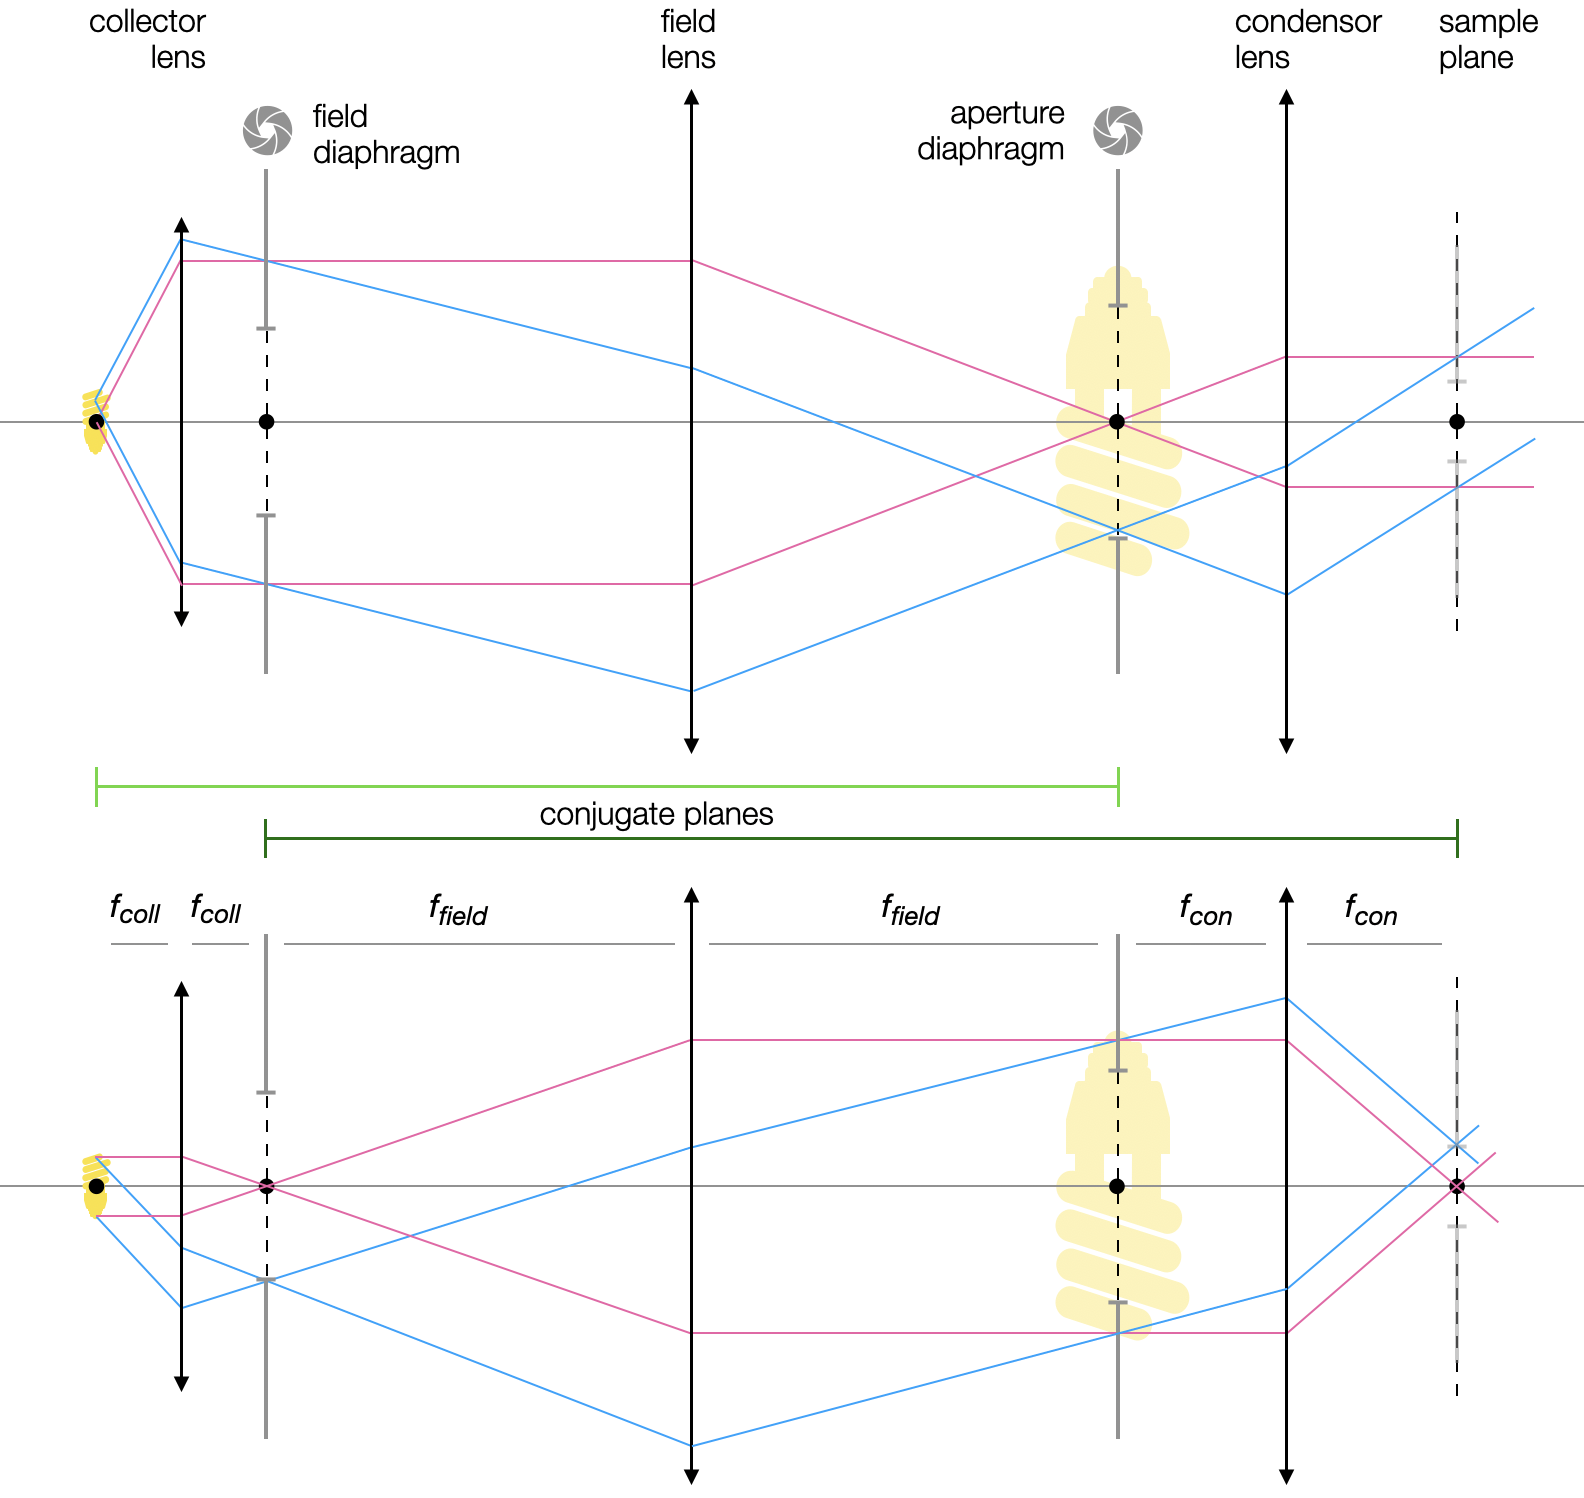
\includegraphics[width=1\textwidth]{figures/koehler_illumination.png}
	\captionsetup{width=0.95\textwidth}
	\caption{K\"{o}hler illumination. \\
	\emph{Top:} Rays are drawn highlighting the infinite conjugate formed by collector and field lens. These rays illustrate i) how each point on the light source illuminates the whole sample, yielding uniform illumination; ii) how the light source is imaged onto the aperture diaphragm with $m=f_{field}/f_{coll}$ (here $m=-5$); iii) how closing the aperture diaphragm shrinks the effective extent of the light source, and hence the angles with which the sample is illuminated, but has no effect on the area of the sample that is illuminated. \\
	\emph{Bottom:} Rays are drawn highlighting the infinite conjugate formed by field and condensor lens. These rays illustrate i) how each point on the sample receives light from all points on the light source; ii) how the field diaphragm is imaged onto the sample plane with $m=f_{con}/f_{field}$ (here m=-2.5); iii) how closing the field diaphragm restricts the area on the sample that is illuminated, but has no effect on the angles of illumination.}
	\label{fig:koehler_illumination}
\end{figure}


\subsubsection{A reminder of the six requirements}
\begin{enumerate}
    \item Bright: You can see that the higher the numerical aperture (NA) of the collector lens, the more light is collected from the LED. $NA=sin(a)$, where $a$ is the half-angle of the maximal cone of light the lens can `collimate' (example: a $50mm$ diameter lens with $f=25mm$ has an $NA=45deg$).
    \item Uniform: Only if the illumination is uniform can we attribute differences in brightness in the image to the structure in the sample. How do we avoid seeing the shape of the light source on the sample? We make sure the light source is `de-focused' on the sample, meaning it is imaged to infinity in the sample plane. The top panel in Fig. \ref{fig:koehler_illumination} illustrates this: each point on the light source illuminates the whole sample.
    \item Angled: This has to do with diffraction orders. Light falling onto the sample diffracts, with finer spatial detail leaving the sample at larger angles. Therefore, the resolution of our imaging system (objective and tube lens) is higher the more angles it can accept - we `reconstruct' the sample using more fine-grained spatial information. Only the zero and first order needs to be captured by the objective (additional orders just increase brightness, but carry no further information about the spatial features contained in that angle). As a consequence, an additional way to increase the resolution of the system is to use angled illumination: this rotates the diffraction orders by the same amount as the illumination, making the zero orders fall away from the centre of the objective. This can effectively double the widest acceptable angle between the zero and first order, if the illumination contains angles of at least the acceptance angle of the objective lens, thus doubling resolution. Under these circumstances, the abbe resolution criterion $\lambda / (2\cdot NA)$ holds.
    \item Control over field of illumination: Light falling on regions of the sample outside of what is imaged by the camera sensor is to be avoided for two reasons. First, it might damage the sample unnecessarily; Second, and more importantly, it can scatter within the sample and enter the objective, not having diffracted from within the imaged area and therefore decreasing contrast (signal to noise so to speak) in the image.
    \item Control over angles: This again relates to diffraction orders and is useful for three reasons. First, from the argument in point 3. follows that illuminating the sample with more extreme angles than given by the NA of the objective does nothing to increase resolution. Therefore, that light is better blocked with the aperture diaphragm to avoid decreasing contrast, for the same reasons given in point 4. Second, while we always want maximal $xy$-resolution, $z$-resolution is not always desirable. High $z$-resolution means a shallow \emph{depth-of-field}, where objects are in focus in a narrow optical plane only -- this means many features will appear blurred on the sensor (unless the sample is cut very thinly). Closing the aperture diaphragm will decrease $z$-resolution, thereby increasing the depth-of-field. Third, see point 6.
    \item Control over brightness: If xy-resolution is not a major concern, closing the aperture allows for control of the intensity of illumination -- it affects all points in the sample equally, reducing the angles of illumination and thus dimming the illumination.
\end{enumerate}

   \noindent
   \hyperlink{hintBack-illumination}{Go back}


\subsubsection{Choosing the right focal lengths}
Fig. \ref{fig:koehler_illumination} helps us reason through this. We need a high NA collector lens so we don't loose too much light. Field and condensor lens are chosen jointly to create enough angles to match the highest NA objective you plan to use. In our case this is the olympus 10x with NA=0.3. The illumination NA depends on three factors: i) the size of the light source; ii) the magnification of the light source by $m=-f_{field}/f_{coll}$; iii) $f_{con}$.

For example, if the emitter is 1mm, magnified 5x to 5mm, then passing through a 50mm condensor lens, this gives $NA=sin(tan(2.5/50))=0.05$. You see with our tiny light source it can be hard to get large angles of illumination. For small angles, $sin(\alpha)\cong\alpha$ and $tan(\alpha)\cong\alpha$, thus doubling the emitter size or $f_{field}$, or halving $f_{con}$, will double the illumination NA.

A reasonable choice given what you have in your kit is $f_{coll}=25mm$, $f_{field}=100mm$ and $f_{con}=60mm$.


   \noindent
   \hyperlink{hintBack-illumination}{Go back}


\subsubsection{Optical alignment tricks}
We can look at Fig. \ref{fig:koehler_illumination} for getting the distances right. A crucial point to keep in mind is that there are two infinite conjugate systems that share the field lens (top and bottom drawing in Fig. \ref{fig:koehler_illumination}).

\begin{itemize}
    \item The collector lens is correctly placed at $f_{coll}$ from the emitter if you can see a large image of the emitter meters away on the wall. This means at $f_{coll}$ after the lens you are very far away from the conjugate plane of the emitter (which is on the wall).
    \item Place the rest of the lenses and diaphragms, using the ruler to measure from the centre of the optics.
    \item Check that at $f_{field}$ after the field lens, you find the image of the emitter (magnified as expected) -- this is where the aperture diaphragm should be placed.
    \item Check that the field diaphragm is in sharp focus in the sample plane, $f_{con}$ from the condensor lens. It should look nicely polygonal. If not, move the diaphragm (this is to avoid moving the field lens, which would make us move the aperture diaphragm). Also, verify the diaphragm is minified as expected.
    \item Check that closing the aperture diaphragm reduces sample illumination, without changing the field of illumination (you should never see an edge creeping in, as shown by the pink rays in the top panel of Fig. \ref{fig:koehler_illumination}). Move the condensor lens to correct.
    \item At the end, check again the two diaphragms operate `orthogonally' to each other, affecting only brightness or only field size.

\end{itemize}

   \noindent
   \hyperlink{hintBack-illumination}{Go back}
   \clearpage

    %----------------------------------------------------------------------
   \subsection{Hint - imaging the sample}
    %----------------------------------------------------------------------
\hypertarget{hintTo-imaging}{}

\subsubsection{A single lens}
You know this from your eyes. And from your cellphone. And from the previous practical. However, microscopes use an infinite conjugate pair to form an image. The reason for this is resolution: the larger the acceptance angle or $NA$ of the lens collecting the diffraction orders from the sample, the higher the resolution (or the more faithful the reconstruction of the sample). If you want to magnify the sample with a single lens, the sample must be placed between $-2f$ and $-1f$ -- this decreases the effective NA of the lens, which is highest if the sample is placed at exactly $1f$. Therefore we use a second lens to form an image.

   \noindent
   \hyperlink{hintBack-imaging}{Go back}

\subsubsection{A question of resolution}
When we ask `can we see it?', we think of separating objects of that size from each other. If there are two cells next to each other, will you see two cells?
Abbe tells us if the effective condensor NA equals the objective NA, we can just distinguish things that are $\lambda / (2NA)$ apart.
For the 4x objective ($NA=0.1$) and $500nm$ light, this gives 2.5$\mu m$ -- surprised?
You just built a microscope! Though is your effective condensor $NA\geq 0.1$?
What can you see with the 10x objective?

   \noindent
   \hyperlink{hintBack-imaging}{Go back}

\subsubsection{Ensuring image formation at 1 WD}
If the tube lens is exactly $1f$ away from the camera sensor, we will see the sample in focus when it is at $1f$ from the objective.
Thus, the tube lens--camera distance must be carefully measured, which is doable since a typical tube lens has a focal length of around 200mm.
To bring the sample into focus, the objective can be moved with respect to the sample, making use of the infinite space between objective and tube lens.
If the objective is switched out for a higher power one (with a shorter focal length), nothing changes on our imaging setup except we re-focus on the sample by moving the objective.
\noindent
\hyperlink{hintBack-imaging}{Go back}
\clearpage
\end{document}
